\section{Motivation}

Satellite-derived data has become a key part of critical infrastructure for private, national, and scientific use.
Although new satellites are being launched at a high rate, even decades-old satellites are seeing novel use cases including advanced forest fire detection~\cite{nasaFirms} and analysis of activities in conflict areas~\cite{separatistLuminosity}. % TODO: cite a new forest fire paper, not FIRMS
These systems were built when robust cryptography was uncommon due to less powerful onboard computers.
It is now well accepted that legacy software which handles data without resilient authentication, such as these terrestrial processing systems, is not resilient against modern adversaries.
However, this was not a practical concern at the time since attacks at the physical layer would have required a costly and highly specialized setup.
Consequently, there does not exist any current work to understand the effects of a modern adversary against such a system.

Recent decades have seen a significant rise in the off-the-shelf availability of software-defined radio hardware, capable of emitting arbitrary signals at a wide range of frequencies.
This lowers the barrier to entry for signal injection attacks significantly~\cite{manulis2021cyber}. % TODO: page 306 (actually 20), top left
Accordingly, satellite systems must now contend with the effects of signal injection, which include poisoning the dataset and exploiting the decoder.
For example, the recent attack against ViaSat's satellite broadband capabilities exploited side channel vulnerabilities in the terrestrial network, resulting in the receiver stations across Ukraine being permanently disabled~\cite{satcomAnalysis}.

Additionally, downstream systems which rely upon datasets are at risk from new supply chain security issues, where the satellite-derived datasets may be compromised.
This includes critical infrastructure for forest fire and storm detection~\cite{nasaFirms,sarikhani2021new}, as well as research organisations and private enterprises.
However, until now there does not exist a classification of these use cases.

\begin{figure}
    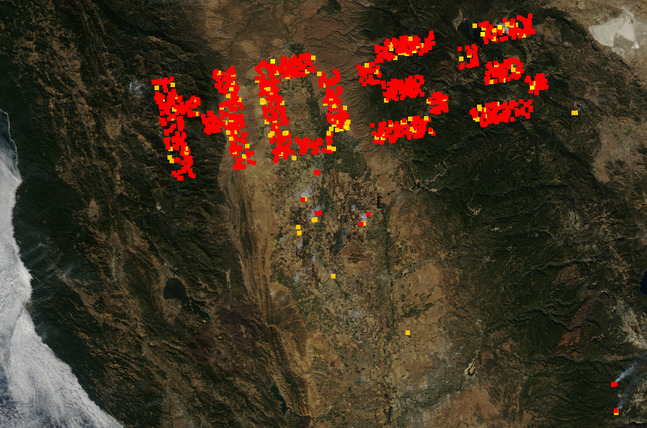
\includegraphics[width=\columnwidth]{diagrams/injection/pixels_800_140.jpg}
    \caption{An injected signal from the attacker manipulates the infrared channels of satellite imagery to create ficticious fires in the resulting dataset.}
    \label{fig:location-injection}
\end{figure}

% key point: Earth observation have scientific instruments that are really expensive

Unfortunately, upgrading existing satellites to use robust cryptography is infeasible and the data is still widely used.
Therefore recent work into anti-spoofing countermeasures depends on analyzing artifacts of overshadowing on the physical channel to determine the authenticity of the received data~\cite{jedermann2021orbit,oligeri2020past}.
Other possible countermeasures include the comparison of data as received at multiple locations, or additional consistency checks.

In this work we therefore analyse the security threat posed by attackers equipped with modern SDR hardware against Earth observing (EO) SATCOM architectures.
In Section~\ref{sec:background}, describe the security properties of common EO SATCOM architectures, and the currently proposed anti-spoofing countermeasures.
We model the adversary in Section~\ref{sec:attack}, drawing out the capabilities required to overshadow an insecure SATCOM link.
In Section~\ref{sec:attack} we consider, through an end-to-end case study, how such an attacker can target NASA's real time forst fire API.
Finally, in Section~\ref{sec:evaluation}, we evaluate the effectiveness of existing countermeasures in detecting and preventing this attack.
% TODO: something about related work?

At the time of writing, we have been in contact with NASA's Direct Readout Laboratory to disclose our findings, and are in the process of compiling a complete vulnerability report.
